\documentclass{standalone}
\usepackage{tikz}
\usetikzlibrary{patterns, positioning}
\usepackage[sfdefault]{ClearSans} %% option 'sfdefault' activates Clear Sans as the default text font
\usepackage[T1]{fontenc}

\begin{document}
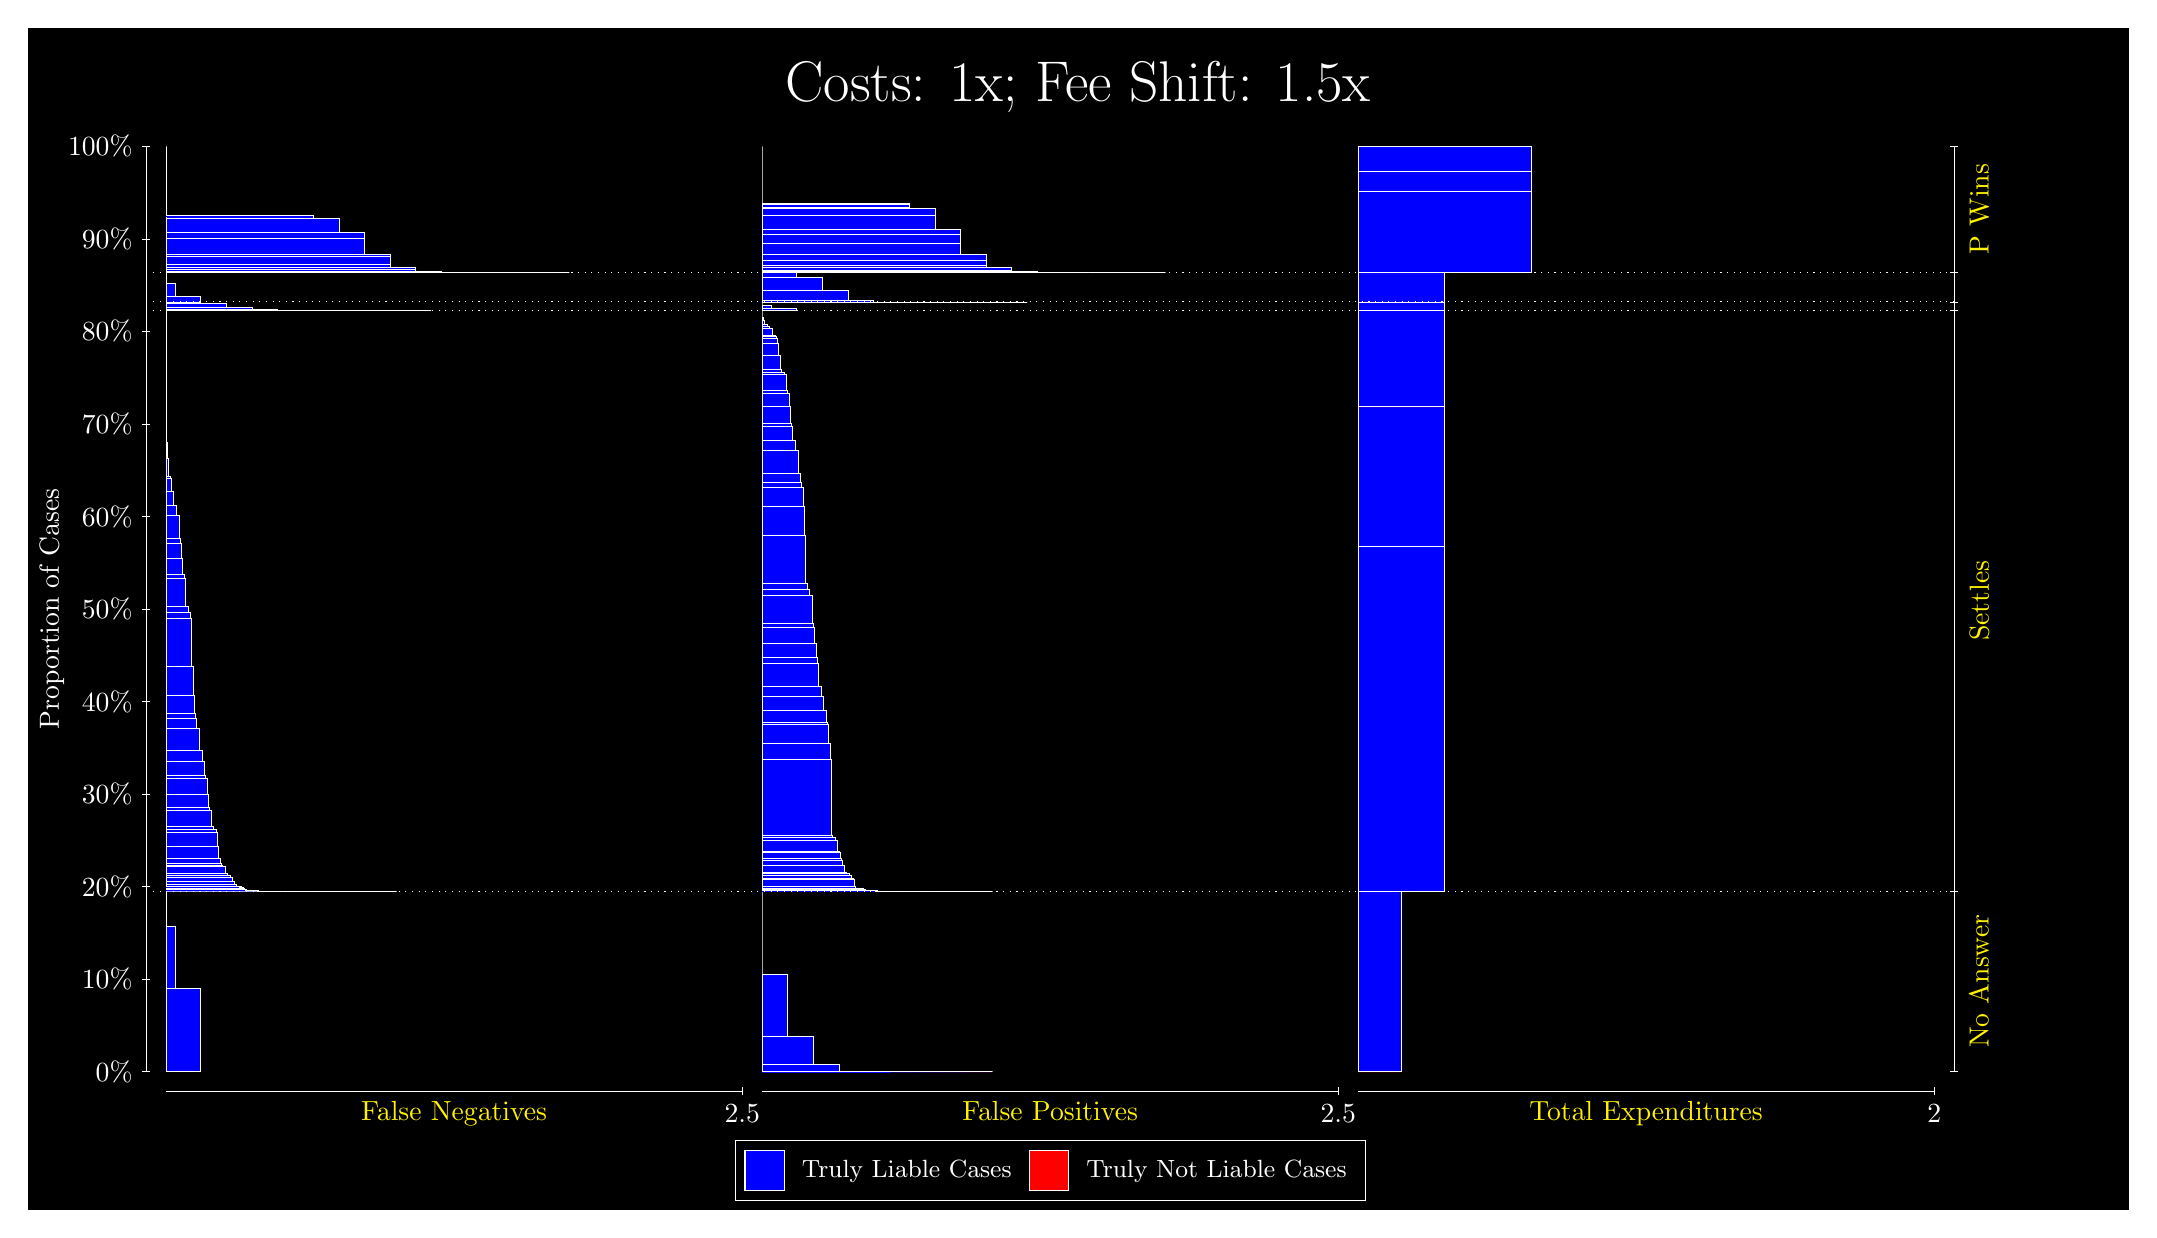
\begin{tikzpicture}
\draw[fill=black] (0,0) rectangle (26.667,15);
\draw[text=white] (0,13.5) rectangle (26.667,15) node[midway] {\huge Costs: 1x; Fee Shift: 1.5x};
\draw[white, very thin] (1.5,1.75) -- (1.5,13.5);
\node[rotate=90, text=white, anchor=center] at (0.3, 7.625) {Proportion of Cases};
\draw[white, very thin] (1.45,1.75) -- (1.55,1.75);
\node[text=white, anchor=east] at (1.45, 1.75) {0\%};
\draw[white, very thin] (1.45,2.925) -- (1.55,2.925);
\node[text=white, anchor=east] at (1.45, 2.925) {10\%};
\draw[white, very thin] (1.45,4.1) -- (1.55,4.1);
\node[text=white, anchor=east] at (1.45, 4.1) {20\%};
\draw[white, very thin] (1.45,5.275) -- (1.55,5.275);
\node[text=white, anchor=east] at (1.45, 5.275) {30\%};
\draw[white, very thin] (1.45,6.45) -- (1.55,6.45);
\node[text=white, anchor=east] at (1.45, 6.45) {40\%};
\draw[white, very thin] (1.45,7.625) -- (1.55,7.625);
\node[text=white, anchor=east] at (1.45, 7.625) {50\%};
\draw[white, very thin] (1.45,8.8) -- (1.55,8.8);
\node[text=white, anchor=east] at (1.45, 8.8) {60\%};
\draw[white, very thin] (1.45,9.975) -- (1.55,9.975);
\node[text=white, anchor=east] at (1.45, 9.975) {70\%};
\draw[white, very thin] (1.45,11.15) -- (1.55,11.15);
\node[text=white, anchor=east] at (1.45, 11.15) {80\%};
\draw[white, very thin] (1.45,12.325) -- (1.55,12.325);
\node[text=white, anchor=east] at (1.45, 12.325) {90\%};
\draw[white, very thin] (1.45,13.5) -- (1.55,13.5);
\node[text=white, anchor=east] at (1.45, 13.5) {100\%};

\draw[white, very thin] (24.457,1.75) -- (24.457,13.5);
\draw[white, very thin] (24.407,1.75) -- (24.507,1.75);
\node[anchor=west] at (24.407, 1.75) {};
\draw[white, very thin] (24.407,4.0413) -- (24.507,4.0413);
\node[anchor=west] at (24.407, 4.0413) {};
\draw[white, very thin] (24.407,11.419) -- (24.507,11.419);
\node[anchor=west] at (24.407, 11.419) {};
\draw[white, very thin] (24.407,11.524) -- (24.507,11.524);
\node[anchor=west] at (24.407, 11.524) {};
\draw[white, very thin] (24.407,11.902) -- (24.507,11.902);
\node[anchor=west] at (24.407, 11.902) {};
\draw[white, very thin] (24.407,13.5) -- (24.507,13.5);
\node[anchor=west] at (24.407, 13.5) {};

\draw[white, very thin, fill=blue] (1.75,1.75) rectangle (2.1891,2.8115);
\draw[white, very thin, fill=blue] (1.75,2.8115) rectangle (1.8638,3.598);
\draw[white, very thin, fill=red] (1.75,3.598) rectangle (1.75,3.598);
\draw[white, very thin, fill=blue] (1.75,3.598) rectangle (1.75,4.0413);
\draw[white, very thin, fill=blue] (1.75,4.0413) rectangle (4.6775,4.0413);
\draw[white, very thin, fill=blue] (1.75,4.0413) rectangle (4.5312,4.0413);
\draw[white, very thin, fill=blue] (1.75,4.0413) rectangle (4.3848,4.0413);
\draw[white, very thin, fill=blue] (1.75,4.0413) rectangle (4.3523,4.0413);
\draw[white, very thin, fill=blue] (1.75,4.0413) rectangle (4.2384,4.0413);
\draw[white, very thin, fill=blue] (1.75,4.0413) rectangle (4.2059,4.0413);
\draw[white, very thin, fill=blue] (1.75,4.0413) rectangle (4.092,4.0413);
\draw[white, very thin, fill=blue] (1.75,4.0413) rectangle (4.0595,4.0413);
\draw[white, very thin, fill=blue] (1.75,4.0413) rectangle (4.027,4.0413);
\draw[white, very thin, fill=blue] (1.75,4.0413) rectangle (3.9457,4.0413);
\draw[white, very thin, fill=blue] (1.75,4.0413) rectangle (3.9131,4.0413);
\draw[white, very thin, fill=blue] (1.75,4.0413) rectangle (3.8806,4.0413);
\draw[white, very thin, fill=blue] (1.75,4.0413) rectangle (3.7993,4.0413);
\draw[white, very thin, fill=blue] (1.75,4.0413) rectangle (3.7668,4.0413);
\draw[white, very thin, fill=blue] (1.75,4.0413) rectangle (3.7342,4.0413);
\draw[white, very thin, fill=blue] (1.75,4.0413) rectangle (3.7017,4.0413);
\draw[white, very thin, fill=blue] (1.75,4.0413) rectangle (3.6529,4.0413);
\draw[white, very thin, fill=blue] (1.75,4.0413) rectangle (3.6204,4.0413);
\draw[white, very thin, fill=blue] (1.75,4.0413) rectangle (3.5878,4.0413);
\draw[white, very thin, fill=blue] (1.75,4.0413) rectangle (3.5553,4.0413);
\draw[white, very thin, fill=blue] (1.75,4.0413) rectangle (3.5065,4.0413);
\draw[white, very thin, fill=blue] (1.75,4.0413) rectangle (3.474,4.0413);
\draw[white, very thin, fill=blue] (1.75,4.0413) rectangle (3.4415,4.0413);
\draw[white, very thin, fill=blue] (1.75,4.0413) rectangle (3.4089,4.0413);
\draw[white, very thin, fill=blue] (1.75,4.0413) rectangle (3.3764,4.0413);
\draw[white, very thin, fill=blue] (1.75,4.0413) rectangle (3.3602,4.0413);
\draw[white, very thin, fill=blue] (1.75,4.0413) rectangle (3.3276,4.0413);
\draw[white, very thin, fill=blue] (1.75,4.0413) rectangle (3.2951,4.0413);
\draw[white, very thin, fill=blue] (1.75,4.0413) rectangle (3.2626,4.0413);
\draw[white, very thin, fill=blue] (1.75,4.0413) rectangle (3.23,4.0413);
\draw[white, very thin, fill=blue] (1.75,4.0413) rectangle (3.2138,4.0413);
\draw[white, very thin, fill=blue] (1.75,4.0413) rectangle (3.1812,4.0413);
\draw[white, very thin, fill=blue] (1.75,4.0413) rectangle (3.1487,4.0414);
\draw[white, very thin, fill=blue] (1.75,4.0414) rectangle (3.1162,4.0414);
\draw[white, very thin, fill=blue] (1.75,4.0414) rectangle (3.0837,4.0414);
\draw[white, very thin, fill=blue] (1.75,4.0414) rectangle (3.0674,4.042);
\draw[white, very thin, fill=blue] (1.75,4.042) rectangle (3.0511,4.0423);
\draw[white, very thin, fill=blue] (1.75,4.0423) rectangle (3.0349,4.0423);
\draw[white, very thin, fill=blue] (1.75,4.0423) rectangle (3.0023,4.0423);
\draw[white, very thin, fill=blue] (1.75,4.0423) rectangle (2.9698,4.0428);
\draw[white, very thin, fill=blue] (1.75,4.0428) rectangle (2.9373,4.0443);
\draw[white, very thin, fill=blue] (1.75,4.0443) rectangle (2.921,4.0486);
\draw[white, very thin, fill=blue] (1.75,4.0486) rectangle (2.9048,4.0488);
\draw[white, very thin, fill=blue] (1.75,4.0488) rectangle (2.8885,4.0494);
\draw[white, very thin, fill=blue] (1.75,4.0494) rectangle (2.856,4.05);
\draw[white, very thin, fill=blue] (1.75,4.05) rectangle (2.8234,4.0548);
\draw[white, very thin, fill=blue] (1.75,4.0548) rectangle (2.7909,4.0552);
\draw[white, very thin, fill=blue] (1.75,4.0552) rectangle (2.7746,4.0583);
\draw[white, very thin, fill=blue] (1.75,4.0583) rectangle (2.7584,4.0613);
\draw[white, very thin, fill=blue] (1.75,4.0613) rectangle (2.7421,4.0777);
\draw[white, very thin, fill=blue] (1.75,4.0777) rectangle (2.7258,4.0933);
\draw[white, very thin, fill=blue] (1.75,4.0933) rectangle (2.7096,4.0964);
\draw[white, very thin, fill=blue] (1.75,4.0964) rectangle (2.6771,4.0981);
\draw[white, very thin, fill=blue] (1.75,4.0981) rectangle (2.6445,4.1223);
\draw[white, very thin, fill=blue] (1.75,4.1223) rectangle (2.6283,4.1311);
\draw[white, very thin, fill=blue] (1.75,4.1311) rectangle (2.612,4.1646);
\draw[white, very thin, fill=blue] (1.75,4.1646) rectangle (2.5957,4.2169);
\draw[white, very thin, fill=blue] (1.75,4.2169) rectangle (2.5795,4.2233);
\draw[white, very thin, fill=blue] (1.75,4.2233) rectangle (2.5632,4.2464);
\draw[white, very thin, fill=blue] (1.75,4.2464) rectangle (2.5307,4.2672);
\draw[white, very thin, fill=blue] (1.75,4.2672) rectangle (2.4982,4.3544);
\draw[white, very thin, fill=blue] (1.75,4.3544) rectangle (2.4656,4.3719);
\draw[white, very thin, fill=blue] (1.75,4.3719) rectangle (2.4494,4.3991);
\draw[white, very thin, fill=blue] (1.75,4.3991) rectangle (2.4331,4.4584);
\draw[white, very thin, fill=blue] (1.75,4.4584) rectangle (2.4168,4.6147);
\draw[white, very thin, fill=blue] (1.75,4.6147) rectangle (2.4006,4.7932);
\draw[white, very thin, fill=blue] (1.75,4.7932) rectangle (2.3843,4.83);
\draw[white, very thin, fill=blue] (1.75,4.83) rectangle (2.3518,4.8584);
\draw[white, very thin, fill=blue] (1.75,4.8584) rectangle (2.3192,5.0643);
\draw[white, very thin, fill=blue] (1.75,5.0643) rectangle (2.303,5.1021);
\draw[white, very thin, fill=blue] (1.75,5.1021) rectangle (2.2867,5.2665);
\draw[white, very thin, fill=blue] (1.75,5.2665) rectangle (2.2705,5.473);
\draw[white, very thin, fill=blue] (1.75,5.473) rectangle (2.2542,5.5103);
\draw[white, very thin, fill=blue] (1.75,5.5103) rectangle (2.2379,5.6964);
\draw[white, very thin, fill=blue] (1.75,5.6964) rectangle (2.2054,5.8252);
\draw[white, very thin, fill=blue] (1.75,5.8252) rectangle (2.1729,6.1096);
\draw[white, very thin, fill=blue] (1.75,6.1096) rectangle (2.1403,6.2332);
\draw[white, very thin, fill=blue] (1.75,6.2332) rectangle (2.1241,6.2936);
\draw[white, very thin, fill=blue] (1.75,6.2936) rectangle (2.1078,6.5274);
\draw[white, very thin, fill=blue] (1.75,6.5274) rectangle (2.0915,6.898);
\draw[white, very thin, fill=blue] (1.75,6.898) rectangle (2.0753,7.5065);
\draw[white, very thin, fill=blue] (1.75,7.5065) rectangle (2.059,7.586);
\draw[white, very thin, fill=blue] (1.75,7.586) rectangle (2.0265,7.6608);
\draw[white, very thin, fill=blue] (1.75,7.6608) rectangle (1.994,8.0199);
\draw[white, very thin, fill=blue] (1.75,8.0199) rectangle (1.9777,8.069);
\draw[white, very thin, fill=blue] (1.75,8.069) rectangle (1.9614,8.2674);
\draw[white, very thin, fill=blue] (1.75,8.2674) rectangle (1.9452,8.4555);
\draw[white, very thin, fill=blue] (1.75,8.4555) rectangle (1.9289,8.5239);
\draw[white, very thin, fill=blue] (1.75,8.5239) rectangle (1.9126,8.8135);
\draw[white, very thin, fill=blue] (1.75,8.8135) rectangle (1.8801,8.9419);
\draw[white, very thin, fill=blue] (1.75,8.9419) rectangle (1.8476,9.121);
\draw[white, very thin, fill=blue] (1.75,9.121) rectangle (1.8151,9.2801);
\draw[white, very thin, fill=blue] (1.75,9.2801) rectangle (1.7988,9.3039);
\draw[white, very thin, fill=blue] (1.75,9.3039) rectangle (1.7825,9.5413);
\draw[white, very thin, fill=blue] (1.75,9.5413) rectangle (1.7663,9.7411);
\draw[white, very thin, fill=red] (1.75,9.7411) rectangle (1.75,9.7411);
\draw[white, very thin, fill=blue] (1.75,9.7411) rectangle (1.75,11.419);
\draw[white, very thin, fill=blue] (1.75,11.419) rectangle (5.1167,11.419);
\draw[white, very thin, fill=blue] (1.75,11.419) rectangle (4.7914,11.419);
\draw[white, very thin, fill=blue] (1.75,11.419) rectangle (4.4661,11.419);
\draw[white, very thin, fill=blue] (1.75,11.419) rectangle (4.1408,11.419);
\draw[white, very thin, fill=blue] (1.75,11.419) rectangle (3.8155,11.419);
\draw[white, very thin, fill=blue] (1.75,11.419) rectangle (3.4903,11.42);
\draw[white, very thin, fill=blue] (1.75,11.42) rectangle (3.165,11.425);
\draw[white, very thin, fill=blue] (1.75,11.425) rectangle (2.8397,11.458);
\draw[white, very thin, fill=blue] (1.75,11.458) rectangle (2.5144,11.504);
\draw[white, very thin, fill=blue] (1.75,11.504) rectangle (2.1891,11.524);
\draw[white, very thin, fill=red] (1.75,11.524) rectangle (1.75,11.524);
\draw[white, very thin, fill=blue] (1.75,11.524) rectangle (2.1891,11.596);
\draw[white, very thin, fill=blue] (1.75,11.596) rectangle (1.8638,11.755);
\draw[white, very thin, fill=red] (1.75,11.755) rectangle (1.75,11.755);
\draw[white, very thin, fill=blue] (1.75,11.755) rectangle (1.75,11.902);
\draw[white, very thin, fill=blue] (1.75,11.902) rectangle (6.8732,11.902);
\draw[white, very thin, fill=blue] (1.75,11.902) rectangle (6.5479,11.902);
\draw[white, very thin, fill=blue] (1.75,11.902) rectangle (6.2226,11.902);
\draw[white, very thin, fill=blue] (1.75,11.902) rectangle (5.8974,11.902);
\draw[white, very thin, fill=blue] (1.75,11.902) rectangle (5.8974,11.902);
\draw[white, very thin, fill=blue] (1.75,11.902) rectangle (5.5721,11.903);
\draw[white, very thin, fill=blue] (1.75,11.903) rectangle (5.5721,11.903);
\draw[white, very thin, fill=blue] (1.75,11.903) rectangle (5.2468,11.913);
\draw[white, very thin, fill=blue] (1.75,11.913) rectangle (4.9215,11.933);
\draw[white, very thin, fill=blue] (1.75,11.933) rectangle (4.9215,11.965);
\draw[white, very thin, fill=blue] (1.75,11.965) rectangle (4.5962,11.997);
\draw[white, very thin, fill=blue] (1.75,11.997) rectangle (4.5962,12.109);
\draw[white, very thin, fill=blue] (1.75,12.109) rectangle (4.5962,12.132);
\draw[white, very thin, fill=blue] (1.75,12.132) rectangle (4.2709,12.334);
\draw[white, very thin, fill=blue] (1.75,12.334) rectangle (4.2709,12.412);
\draw[white, very thin, fill=blue] (1.75,12.412) rectangle (3.9457,12.589);
\draw[white, very thin, fill=blue] (1.75,12.589) rectangle (3.6204,12.591);
\draw[white, very thin, fill=blue] (1.75,12.591) rectangle (3.6204,12.619);
\draw[white, very thin, fill=blue] (1.75,12.619) rectangle (3.5878,12.619);
\draw[white, very thin, fill=blue] (1.75,12.619) rectangle (3.2951,12.62);
\draw[white, very thin, fill=blue] (1.75,12.62) rectangle (3.2951,12.62);
\draw[white, very thin, fill=blue] (1.75,12.62) rectangle (3.2626,12.62);
\draw[white, very thin, fill=blue] (1.75,12.62) rectangle (3.2626,12.62);
\draw[white, very thin, fill=blue] (1.75,12.62) rectangle (2.9698,12.62);
\draw[white, very thin, fill=blue] (1.75,12.62) rectangle (2.9698,12.62);
\draw[white, very thin, fill=blue] (1.75,12.62) rectangle (2.9373,12.62);
\draw[white, very thin, fill=blue] (1.75,12.62) rectangle (2.9373,12.62);
\draw[white, very thin, fill=blue] (1.75,12.62) rectangle (2.9373,12.62);
\draw[white, very thin, fill=blue] (1.75,12.62) rectangle (2.6445,12.62);
\draw[white, very thin, fill=blue] (1.75,12.62) rectangle (2.6445,12.62);
\draw[white, very thin, fill=blue] (1.75,12.62) rectangle (2.612,12.62);
\draw[white, very thin, fill=blue] (1.75,12.62) rectangle (2.612,12.62);
\draw[white, very thin, fill=blue] (1.75,12.62) rectangle (2.3192,12.62);
\draw[white, very thin, fill=blue] (1.75,12.62) rectangle (2.3192,12.62);
\draw[white, very thin, fill=blue] (1.75,12.62) rectangle (2.2867,12.62);
\draw[white, very thin, fill=blue] (1.75,12.62) rectangle (2.2867,12.62);
\draw[white, very thin, fill=blue] (1.75,12.62) rectangle (2.2867,12.62);
\draw[white, very thin, fill=blue] (1.75,12.62) rectangle (1.994,12.62);
\draw[white, very thin, fill=blue] (1.75,12.62) rectangle (1.994,12.62);
\draw[white, very thin, fill=blue] (1.75,12.62) rectangle (1.9614,12.621);
\draw[white, very thin, fill=blue] (1.75,12.621) rectangle (1.9614,12.621);
\draw[white, very thin, fill=blue] (1.75,12.621) rectangle (1.9614,12.624);
\draw[white, very thin, fill=red] (1.75,12.624) rectangle (1.75,12.624);
\draw[white, very thin, fill=blue] (1.75,12.624) rectangle (1.75,13.5);
\draw[white, very thin, fill=red] (9.3189,1.75) rectangle (12.246,1.75);
\draw[white, very thin, fill=blue] (9.3189,1.75) rectangle (12.246,1.75);
\draw[white, very thin, fill=blue] (9.3189,1.75) rectangle (11.921,1.75);
\draw[white, very thin, fill=blue] (9.3189,1.75) rectangle (11.596,1.75);
\draw[white, very thin, fill=blue] (9.3189,1.75) rectangle (11.271,1.75);
\draw[white, very thin, fill=blue] (9.3189,1.75) rectangle (10.945,1.7503);
\draw[white, very thin, fill=blue] (9.3189,1.7503) rectangle (10.62,1.7576);
\draw[white, very thin, fill=blue] (9.3189,1.7576) rectangle (10.295,1.8358);
\draw[white, very thin, fill=blue] (9.3189,1.8358) rectangle (9.9694,2.1933);
\draw[white, very thin, fill=blue] (9.3189,2.1933) rectangle (9.6442,2.9798);
\draw[white, very thin, fill=blue] (9.3189,2.9798) rectangle (9.3189,4.0413);
\draw[white, very thin, fill=red] (9.3189,4.0413) rectangle (12.246,4.0413);
\draw[white, very thin, fill=blue] (9.3189,4.0413) rectangle (12.246,4.0413);
\draw[white, very thin, fill=red] (9.3189,4.0413) rectangle (12.1,4.0413);
\draw[white, very thin, fill=blue] (9.3189,4.0413) rectangle (12.1,4.0413);
\draw[white, very thin, fill=red] (9.3189,4.0413) rectangle (11.954,4.0413);
\draw[white, very thin, fill=blue] (9.3189,4.0413) rectangle (11.954,4.0413);
\draw[white, very thin, fill=blue] (9.3189,4.0413) rectangle (11.921,4.0413);
\draw[white, very thin, fill=red] (9.3189,4.0413) rectangle (11.807,4.0413);
\draw[white, very thin, fill=blue] (9.3189,4.0413) rectangle (11.807,4.0413);
\draw[white, very thin, fill=blue] (9.3189,4.0413) rectangle (11.775,4.0413);
\draw[white, very thin, fill=red] (9.3189,4.0413) rectangle (11.661,4.0413);
\draw[white, very thin, fill=blue] (9.3189,4.0413) rectangle (11.661,4.0413);
\draw[white, very thin, fill=blue] (9.3189,4.0413) rectangle (11.628,4.0413);
\draw[white, very thin, fill=blue] (9.3189,4.0413) rectangle (11.596,4.0413);
\draw[white, very thin, fill=red] (9.3189,4.0413) rectangle (11.515,4.0413);
\draw[white, very thin, fill=blue] (9.3189,4.0413) rectangle (11.515,4.0413);
\draw[white, very thin, fill=blue] (9.3189,4.0413) rectangle (11.482,4.0413);
\draw[white, very thin, fill=blue] (9.3189,4.0413) rectangle (11.449,4.0413);
\draw[white, very thin, fill=red] (9.3189,4.0413) rectangle (11.368,4.0413);
\draw[white, very thin, fill=blue] (9.3189,4.0413) rectangle (11.368,4.0413);
\draw[white, very thin, fill=blue] (9.3189,4.0413) rectangle (11.336,4.0413);
\draw[white, very thin, fill=blue] (9.3189,4.0413) rectangle (11.303,4.0413);
\draw[white, very thin, fill=blue] (9.3189,4.0413) rectangle (11.271,4.0413);
\draw[white, very thin, fill=red] (9.3189,4.0413) rectangle (11.222,4.0413);
\draw[white, very thin, fill=blue] (9.3189,4.0413) rectangle (11.222,4.0413);
\draw[white, very thin, fill=blue] (9.3189,4.0413) rectangle (11.189,4.0413);
\draw[white, very thin, fill=blue] (9.3189,4.0413) rectangle (11.157,4.0413);
\draw[white, very thin, fill=blue] (9.3189,4.0413) rectangle (11.124,4.0413);
\draw[white, very thin, fill=red] (9.3189,4.0413) rectangle (11.075,4.0413);
\draw[white, very thin, fill=blue] (9.3189,4.0413) rectangle (11.075,4.0413);
\draw[white, very thin, fill=blue] (9.3189,4.0413) rectangle (11.043,4.0413);
\draw[white, very thin, fill=blue] (9.3189,4.0413) rectangle (11.01,4.0414);
\draw[white, very thin, fill=blue] (9.3189,4.0414) rectangle (10.978,4.0414);
\draw[white, very thin, fill=blue] (9.3189,4.0414) rectangle (10.945,4.0414);
\draw[white, very thin, fill=red] (9.3189,4.0414) rectangle (10.929,4.0414);
\draw[white, very thin, fill=blue] (9.3189,4.0414) rectangle (10.929,4.0418);
\draw[white, very thin, fill=blue] (9.3189,4.0418) rectangle (10.896,4.0418);
\draw[white, very thin, fill=blue] (9.3189,4.0418) rectangle (10.864,4.0419);
\draw[white, very thin, fill=blue] (9.3189,4.0419) rectangle (10.831,4.0423);
\draw[white, very thin, fill=blue] (9.3189,4.0423) rectangle (10.799,4.0423);
\draw[white, very thin, fill=red] (9.3189,4.0423) rectangle (10.783,4.0423);
\draw[white, very thin, fill=blue] (9.3189,4.0423) rectangle (10.783,4.0461);
\draw[white, very thin, fill=blue] (9.3189,4.0461) rectangle (10.75,4.0466);
\draw[white, very thin, fill=blue] (9.3189,4.0466) rectangle (10.718,4.0472);
\draw[white, very thin, fill=blue] (9.3189,4.0472) rectangle (10.685,4.052);
\draw[white, very thin, fill=blue] (9.3189,4.052) rectangle (10.653,4.0533);
\draw[white, very thin, fill=red] (9.3189,4.0533) rectangle (10.636,4.0533);
\draw[white, very thin, fill=blue] (9.3189,4.0533) rectangle (10.636,4.0635);
\draw[white, very thin, fill=blue] (9.3189,4.0635) rectangle (10.62,4.0642);
\draw[white, very thin, fill=blue] (9.3189,4.0642) rectangle (10.604,4.0775);
\draw[white, very thin, fill=blue] (9.3189,4.0775) rectangle (10.571,4.0801);
\draw[white, very thin, fill=blue] (9.3189,4.0801) rectangle (10.539,4.0819);
\draw[white, very thin, fill=blue] (9.3189,4.0819) rectangle (10.506,4.1045);
\draw[white, very thin, fill=red] (9.3189,4.1045) rectangle (10.49,4.1045);
\draw[white, very thin, fill=blue] (9.3189,4.1045) rectangle (10.49,4.1965);
\draw[white, very thin, fill=blue] (9.3189,4.1965) rectangle (10.474,4.198);
\draw[white, very thin, fill=blue] (9.3189,4.198) rectangle (10.457,4.242);
\draw[white, very thin, fill=blue] (9.3189,4.242) rectangle (10.425,4.264);
\draw[white, very thin, fill=blue] (9.3189,4.264) rectangle (10.392,4.2845);
\draw[white, very thin, fill=blue] (9.3189,4.2845) rectangle (10.36,4.3718);
\draw[white, very thin, fill=red] (9.3189,4.3718) rectangle (10.344,4.3718);
\draw[white, very thin, fill=blue] (9.3189,4.3718) rectangle (10.344,4.4281);
\draw[white, very thin, fill=blue] (9.3189,4.4281) rectangle (10.327,4.4637);
\draw[white, very thin, fill=blue] (9.3189,4.4637) rectangle (10.311,4.5339);
\draw[white, very thin, fill=blue] (9.3189,4.5339) rectangle (10.295,4.5478);
\draw[white, very thin, fill=blue] (9.3189,4.5478) rectangle (10.278,4.6868);
\draw[white, very thin, fill=blue] (9.3189,4.6868) rectangle (10.246,4.7201);
\draw[white, very thin, fill=blue] (9.3189,4.7201) rectangle (10.213,4.7496);
\draw[white, very thin, fill=red] (9.3189,4.7496) rectangle (10.197,4.7496);
\draw[white, very thin, fill=blue] (9.3189,4.7496) rectangle (10.197,5.7196);
\draw[white, very thin, fill=blue] (9.3189,5.7196) rectangle (10.181,5.9194);
\draw[white, very thin, fill=blue] (9.3189,5.9194) rectangle (10.165,6.1568);
\draw[white, very thin, fill=blue] (9.3189,6.1568) rectangle (10.148,6.1806);
\draw[white, very thin, fill=blue] (9.3189,6.1806) rectangle (10.132,6.3397);
\draw[white, very thin, fill=blue] (9.3189,6.3397) rectangle (10.1,6.5188);
\draw[white, very thin, fill=blue] (9.3189,6.5188) rectangle (10.067,6.6472);
\draw[white, very thin, fill=blue] (9.3189,6.6472) rectangle (10.034,6.9368);
\draw[white, very thin, fill=blue] (9.3189,6.9368) rectangle (10.018,7.0052);
\draw[white, very thin, fill=blue] (9.3189,7.0052) rectangle (10.002,7.1933);
\draw[white, very thin, fill=blue] (9.3189,7.1933) rectangle (9.9857,7.3917);
\draw[white, very thin, fill=blue] (9.3189,7.3917) rectangle (9.9694,7.4408);
\draw[white, very thin, fill=blue] (9.3189,7.4408) rectangle (9.9532,7.7999);
\draw[white, very thin, fill=blue] (9.3189,7.7999) rectangle (9.9206,7.8747);
\draw[white, very thin, fill=blue] (9.3189,7.8747) rectangle (9.8881,7.9542);
\draw[white, very thin, fill=blue] (9.3189,7.9542) rectangle (9.8718,8.5627);
\draw[white, very thin, fill=blue] (9.3189,8.5627) rectangle (9.8556,8.9333);
\draw[white, very thin, fill=blue] (9.3189,8.9333) rectangle (9.8393,9.1671);
\draw[white, very thin, fill=blue] (9.3189,9.1671) rectangle (9.8231,9.2275);
\draw[white, very thin, fill=blue] (9.3189,9.2275) rectangle (9.8068,9.3511);
\draw[white, very thin, fill=blue] (9.3189,9.3511) rectangle (9.7743,9.6355);
\draw[white, very thin, fill=blue] (9.3189,9.6355) rectangle (9.7417,9.7643);
\draw[white, very thin, fill=blue] (9.3189,9.7643) rectangle (9.7092,9.9504);
\draw[white, very thin, fill=blue] (9.3189,9.9504) rectangle (9.6929,9.9877);
\draw[white, very thin, fill=blue] (9.3189,9.9877) rectangle (9.6767,10.194);
\draw[white, very thin, fill=blue] (9.3189,10.194) rectangle (9.6604,10.359);
\draw[white, very thin, fill=blue] (9.3189,10.359) rectangle (9.6442,10.396);
\draw[white, very thin, fill=blue] (9.3189,10.396) rectangle (9.6279,10.602);
\draw[white, very thin, fill=blue] (9.3189,10.602) rectangle (9.5954,10.631);
\draw[white, very thin, fill=blue] (9.3189,10.631) rectangle (9.5628,10.667);
\draw[white, very thin, fill=blue] (9.3189,10.667) rectangle (9.5466,10.846);
\draw[white, very thin, fill=blue] (9.3189,10.846) rectangle (9.5303,11.002);
\draw[white, very thin, fill=blue] (9.3189,11.002) rectangle (9.514,11.062);
\draw[white, very thin, fill=blue] (9.3189,11.062) rectangle (9.4978,11.089);
\draw[white, very thin, fill=blue] (9.3189,11.089) rectangle (9.4815,11.106);
\draw[white, very thin, fill=blue] (9.3189,11.106) rectangle (9.449,11.193);
\draw[white, very thin, fill=blue] (9.3189,11.193) rectangle (9.4165,11.214);
\draw[white, very thin, fill=blue] (9.3189,11.214) rectangle (9.3839,11.237);
\draw[white, very thin, fill=blue] (9.3189,11.237) rectangle (9.3677,11.244);
\draw[white, very thin, fill=blue] (9.3189,11.244) rectangle (9.3514,11.296);
\draw[white, very thin, fill=blue] (9.3189,11.296) rectangle (9.3351,11.33);
\draw[white, very thin, fill=blue] (9.3189,11.33) rectangle (9.3189,11.419);
\draw[white, very thin, fill=red] (9.3189,11.419) rectangle (9.758,11.419);
\draw[white, very thin, fill=blue] (9.3189,11.419) rectangle (9.758,11.44);
\draw[white, very thin, fill=blue] (9.3189,11.44) rectangle (9.4327,11.486);
\draw[white, very thin, fill=blue] (9.3189,11.486) rectangle (9.3189,11.524);
\draw[white, very thin, fill=red] (9.3189,11.524) rectangle (12.686,11.524);
\draw[white, very thin, fill=blue] (9.3189,11.524) rectangle (12.686,11.524);
\draw[white, very thin, fill=blue] (9.3189,11.524) rectangle (12.36,11.524);
\draw[white, very thin, fill=blue] (9.3189,11.524) rectangle (12.035,11.524);
\draw[white, very thin, fill=blue] (9.3189,11.524) rectangle (11.71,11.524);
\draw[white, very thin, fill=blue] (9.3189,11.524) rectangle (11.384,11.524);
\draw[white, very thin, fill=blue] (9.3189,11.524) rectangle (11.059,11.525);
\draw[white, very thin, fill=blue] (9.3189,11.525) rectangle (10.734,11.549);
\draw[white, very thin, fill=blue] (9.3189,11.549) rectangle (10.409,11.672);
\draw[white, very thin, fill=blue] (9.3189,11.672) rectangle (10.083,11.831);
\draw[white, very thin, fill=blue] (9.3189,11.831) rectangle (9.758,11.902);
\draw[white, very thin, fill=red] (9.3189,11.902) rectangle (14.442,11.902);
\draw[white, very thin, fill=blue] (9.3189,11.902) rectangle (14.442,11.902);
\draw[white, very thin, fill=red] (9.3189,11.902) rectangle (14.117,11.902);
\draw[white, very thin, fill=blue] (9.3189,11.902) rectangle (14.117,11.902);
\draw[white, very thin, fill=red] (9.3189,11.902) rectangle (13.792,11.902);
\draw[white, very thin, fill=blue] (9.3189,11.902) rectangle (13.792,11.902);
\draw[white, very thin, fill=blue] (9.3189,11.902) rectangle (13.466,11.902);
\draw[white, very thin, fill=red] (9.3189,11.902) rectangle (13.466,11.902);
\draw[white, very thin, fill=blue] (9.3189,11.902) rectangle (13.466,11.902);
\draw[white, very thin, fill=red] (9.3189,11.902) rectangle (13.141,11.902);
\draw[white, very thin, fill=blue] (9.3189,11.902) rectangle (13.141,11.903);
\draw[white, very thin, fill=blue] (9.3189,11.903) rectangle (13.141,11.903);
\draw[white, very thin, fill=red] (9.3189,11.903) rectangle (12.816,11.903);
\draw[white, very thin, fill=blue] (9.3189,11.903) rectangle (12.816,11.911);
\draw[white, very thin, fill=blue] (9.3189,11.911) rectangle (12.816,11.912);
\draw[white, very thin, fill=blue] (9.3189,11.912) rectangle (12.49,11.928);
\draw[white, very thin, fill=red] (9.3189,11.928) rectangle (12.49,11.928);
\draw[white, very thin, fill=blue] (9.3189,11.928) rectangle (12.49,11.963);
\draw[white, very thin, fill=blue] (9.3189,11.963) rectangle (12.165,11.985);
\draw[white, very thin, fill=red] (9.3189,11.985) rectangle (12.165,11.985);
\draw[white, very thin, fill=blue] (9.3189,11.985) rectangle (12.165,12.057);
\draw[white, very thin, fill=blue] (9.3189,12.057) rectangle (12.165,12.132);
\draw[white, very thin, fill=blue] (9.3189,12.132) rectangle (11.84,12.267);
\draw[white, very thin, fill=blue] (9.3189,12.267) rectangle (11.84,12.389);
\draw[white, very thin, fill=blue] (9.3189,12.389) rectangle (11.84,12.448);
\draw[white, very thin, fill=blue] (9.3189,12.448) rectangle (11.515,12.62);
\draw[white, very thin, fill=blue] (9.3189,12.62) rectangle (11.515,12.711);
\draw[white, very thin, fill=blue] (9.3189,12.711) rectangle (11.189,12.726);
\draw[white, very thin, fill=blue] (9.3189,12.726) rectangle (11.189,12.766);
\draw[white, very thin, fill=blue] (9.3189,12.766) rectangle (11.189,12.778);
\draw[white, very thin, fill=red] (9.3189,12.778) rectangle (11.157,12.778);
\draw[white, very thin, fill=blue] (9.3189,12.778) rectangle (11.157,12.778);
\draw[white, very thin, fill=blue] (9.3189,12.778) rectangle (10.864,12.78);
\draw[white, very thin, fill=blue] (9.3189,12.78) rectangle (10.864,12.783);
\draw[white, very thin, fill=red] (9.3189,12.783) rectangle (10.831,12.783);
\draw[white, very thin, fill=blue] (9.3189,12.783) rectangle (10.831,12.783);
\draw[white, very thin, fill=blue] (9.3189,12.783) rectangle (10.539,12.783);
\draw[white, very thin, fill=blue] (9.3189,12.783) rectangle (10.539,12.783);
\draw[white, very thin, fill=blue] (9.3189,12.783) rectangle (10.539,12.783);
\draw[white, very thin, fill=red] (9.3189,12.783) rectangle (10.506,12.783);
\draw[white, very thin, fill=blue] (9.3189,12.783) rectangle (10.506,12.783);
\draw[white, very thin, fill=blue] (9.3189,12.783) rectangle (10.506,12.783);
\draw[white, very thin, fill=blue] (9.3189,12.783) rectangle (10.506,12.783);
\draw[white, very thin, fill=blue] (9.3189,12.783) rectangle (10.213,12.783);
\draw[white, very thin, fill=blue] (9.3189,12.783) rectangle (10.213,12.783);
\draw[white, very thin, fill=blue] (9.3189,12.783) rectangle (10.181,12.783);
\draw[white, very thin, fill=red] (9.3189,12.783) rectangle (10.181,12.783);
\draw[white, very thin, fill=blue] (9.3189,12.783) rectangle (10.181,12.783);
\draw[white, very thin, fill=blue] (9.3189,12.783) rectangle (10.181,12.783);
\draw[white, very thin, fill=blue] (9.3189,12.783) rectangle (9.8881,12.783);
\draw[white, very thin, fill=blue] (9.3189,12.783) rectangle (9.8556,12.783);
\draw[white, very thin, fill=red] (9.3189,12.783) rectangle (9.8556,12.783);
\draw[white, very thin, fill=blue] (9.3189,12.783) rectangle (9.8556,12.783);
\draw[white, very thin, fill=blue] (9.3189,12.783) rectangle (9.8556,12.783);
\draw[white, very thin, fill=blue] (9.3189,12.783) rectangle (9.5628,12.783);
\draw[white, very thin, fill=blue] (9.3189,12.783) rectangle (9.5628,12.783);
\draw[white, very thin, fill=blue] (9.3189,12.783) rectangle (9.5303,12.783);
\draw[white, very thin, fill=red] (9.3189,12.783) rectangle (9.5303,12.783);
\draw[white, very thin, fill=blue] (9.3189,12.783) rectangle (9.5303,12.783);
\draw[white, very thin, fill=blue] (9.3189,12.783) rectangle (9.5303,12.783);
\draw[white, very thin, fill=red] (9.3189,12.783) rectangle (9.3189,12.783);
\draw[white, very thin, fill=blue] (9.3189,12.783) rectangle (9.3189,13.5);
\draw[white, very thin, fill=red] (16.888,1.75) rectangle (17.437,1.75);
\draw[white, very thin, fill=blue] (16.888,1.75) rectangle (17.437,4.0413);
\draw[white, very thin, fill=red] (16.888,4.0413) rectangle (17.986,4.0413);
\draw[white, very thin, fill=blue] (16.888,4.0413) rectangle (17.986,8.4216);
\draw[white, very thin, fill=red] (16.888,8.4216) rectangle (17.986,8.4216);
\draw[white, very thin, fill=blue] (16.888,8.4216) rectangle (17.986,10.194);
\draw[white, very thin, fill=red] (16.888,10.194) rectangle (17.986,10.194);
\draw[white, very thin, fill=blue] (16.888,10.194) rectangle (17.986,11.419);
\draw[white, very thin, fill=red] (16.888,11.419) rectangle (17.986,11.419);
\draw[white, very thin, fill=blue] (16.888,11.419) rectangle (17.986,11.524);
\draw[white, very thin, fill=red] (16.888,11.524) rectangle (17.986,11.524);
\draw[white, very thin, fill=blue] (16.888,11.524) rectangle (17.986,11.902);
\draw[white, very thin, fill=red] (16.888,11.902) rectangle (19.083,11.902);
\draw[white, very thin, fill=blue] (16.888,11.902) rectangle (19.083,12.933);
\draw[white, very thin, fill=red] (16.888,12.933) rectangle (19.083,12.933);
\draw[white, very thin, fill=blue] (16.888,12.933) rectangle (19.083,13.184);
\draw[white, very thin, fill=red] (16.888,13.184) rectangle (19.083,13.184);
\draw[white, very thin, fill=blue] (16.888,13.184) rectangle (19.083,13.5);
\draw[white, dotted] (1.5,4.0413) -- (24.457,4.0413);
\draw[white, dotted] (1.5,11.419) -- (24.457,11.419);
\draw[white, dotted] (1.5,11.524) -- (24.457,11.524);
\draw[white, dotted] (1.5,11.902) -- (24.457,11.902);
\draw[white, very thin] (1.75,1.5) -- (9.0689,1.5);
\node[text=yellow, anchor=north] at (5.4094, 1.5) {False Negatives};
\draw[white, very thin] (9.0689,1.45) -- (9.0689,1.55);
\node[text=white, anchor=north] at (9.0689, 1.45) {2.5};

\draw[white, very thin] (9.3189,1.5) -- (16.638,1.5);
\node[text=yellow, anchor=north] at (12.978, 1.5) {False Positives};
\draw[white, very thin] (16.638,1.45) -- (16.638,1.55);
\node[text=white, anchor=north] at (16.638, 1.45) {2.5};

\draw[white, very thin] (16.888,1.5) -- (24.207,1.5);
\node[text=yellow, anchor=north] at (20.547, 1.5) {Total Expenditures};
\draw[white, very thin] (24.207,1.45) -- (24.207,1.55);
\node[text=white, anchor=north] at (24.207, 1.45) {2};

\node[text=yellow, centered, rotate=90] at (24.777, 2.8957) {No Answer};
\node[text=yellow, centered, rotate=90] at (24.777, 7.7304) {Settles};


\node[text=yellow, centered, rotate=90] at (24.777, 12.701) {P Wins};

\draw (12.978300999999998,1.5) node[draw=none] (baseCoordinate) {};
\begin{scope}[align=center]
        \matrix[scale=0.5, draw=white, below=0.5cm of baseCoordinate, nodes={draw}, column sep=0.1cm]{
            \node[rectangle, draw, minimum width=0.5cm, minimum height=0.5cm, fill=blue] {}; &
            \node[draw=none, font=\small, text=white] (B) {Truly Liable Cases}; &
            \node[rectangle, draw, minimum width=0.5cm, minimum height=0.5cm, fill=red] {}; &
            \node[draw=none, font=\small, text=white] (B) {Truly Not Liable Cases}; \\
            };
\end{scope}

\end{tikzpicture}
\end{document}